\documentclass{article}
% Language setting
\usepackage[english]{babel}
% Set page size and margins
\usepackage[a4paper,top=2cm,bottom=2cm,left=3cm,right=3cm,marginparwidth=1.75cm]{geometry}
% Other useful packages
\usepackage{xcolor}
\usepackage{amsmath}
\usepackage{graphicx}
\usepackage{hyperref}
\usepackage{minted}
\usepackage{caption}
\usepackage{subcaption}
\urlstyle{same}
%\captionsetup[plain]{skip=-5pt} % move the caption 5 pt above

% package for pseudocode
\usepackage{clrscode3e}

\renewcommand{\listingscaption}{Code} % Use "Code" as caption title
\renewcommand{\listoflistingscaption}{List of \lstlistingname s} % List of Listings -> List of Codes

\renewcommand\theFancyVerbLine{\small\arabic{FancyVerbLine}} % small minted line numbers

\title{\textbf{The convex hull}}
\author{Domenico Ferraro\\\href{mailto:d.ferraro7@studenti.unipi.it}{d.ferraro7@studenti.unipi.it}}

\makeatletter
\hypersetup{
    colorlinks=true,
    linkcolor=black,
    filecolor=black,      
    urlcolor=black,
    citecolor=black,
    anchorcolor=black,
    pdftitle=\@title,
    pdfpagemode=FullScreen, % Determines how the file is opened
    pdfauthor={Domenico Ferraro}
}
\makeatother

\begin{document}

%\maketitle
\vbox{
    \centering
    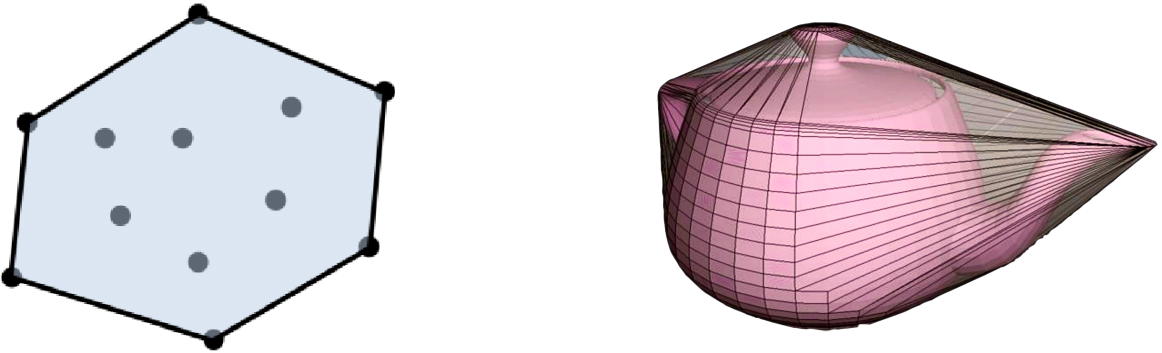
\includegraphics[width=0.5\textwidth]{./cover.jpg}
    %\qquad %inserts a space of 2em
    %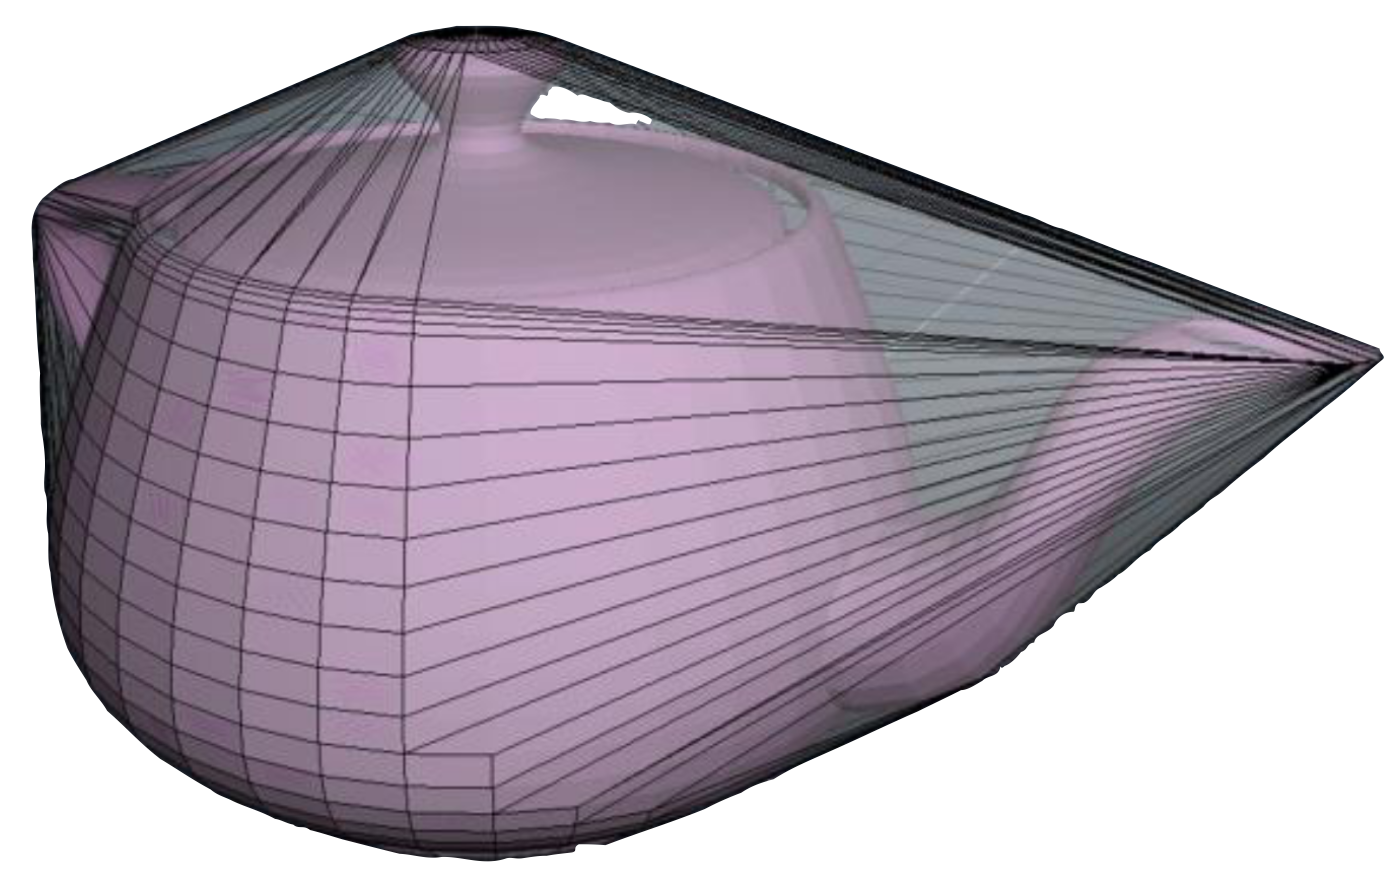
\includegraphics[width=0.25\textwidth]{./3dconvexhull.png}
    \maketitle %this typesets the contents of \title, \author and \date
}
\begin{abstract}
Given a set of points, a convex hull is the subset of points that forms the smallest convex polytope which encloses all the points in the set. Computing the convex hull is a problem in computational geometry and a number of algorithms have been developed to compute it. This report describes the main algorithms to compute the convex hull in 2D, 3D and N-dimensions. For each algorithm we will look at the pseudocode, a running example to visualize how the algorithm works and finally a C++ implementation. We will also solve some competitive programming problems that involves the convex hull. 
\end{abstract}

\tableofcontents

\newpage
\section{Introduction}
In geometry, the convex hull of a set of N-dimensional points is the smallest subset of points that forms the smallest convex polytope which encloses all the points in the set. The convex hull in 2-dimensions is a convex polygon, which is the 2D example of a polytope. We call a shape convex, if for any two points that are inside the shape, the segment between these two points is also inside the shape.

The convex hull is one of the first problems that was studied in computational geometry and the algorithmic problem is fundamental for it. Convex hulls have wide applications in mathematics, statistics, combinatorial optimization, economics, geometric modeling, and ethology.

\subsection{General cases}
It is possible to generalize the problem of finding the convex hull of a set of points in N-dimensions into three general cases:
- the convex hull of a single point or two points
- the convex hull of three points
- the convex hull of $n > 3$ points

Computing the convex hull of a single point or two points is trivial because the convex hull is just the given set of points. Computing the convex hull of three points differs if the points are stored in clockwise order or counter-clockwise order.

Given three points, $a$, $b$, and $c$, the order of the points can be checked by computing the cross-product of the two vectors $(b_x, b_y) - (a_x, a_y)$ and $(c_x, c_y) - (a_x, a_y)$, which is defined as a 2 × 2 determinant:

\begin{center}\textit{counter-clockwise}$ \iff \begin{bmatrix}
b_x - a_x & b_y - a_y\\
c_x - a_x & c_y - a_y
\end{bmatrix} > 0$
\end{center}

\begin{figure}[h]
    \centering
    \begin{subfigure}[b]{.2\linewidth}
        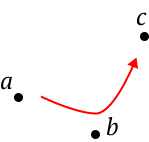
\includegraphics[width=\textwidth]{intro/ccw_test_a.png}
        \caption{\label{fig:ccw_test_a}}
    \end{subfigure}
    \hspace{14mm}
    \begin{subfigure}[b]{.2\linewidth}
        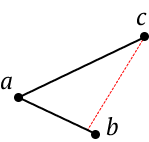
\includegraphics[width=\textwidth]{intro/ccw_test_b.png}
        \caption{\label{fig:ccw_test_b}}
    \end{subfigure}
    
    \caption{\label{fig:ccw_test}Example of three points in counter-clockwise order $(a)$. As can be seen, the cross product is positive $(b)$.}
\end{figure}

Computing the convex hull of $n > 3$ points is not as trivial as the previous cases and it is needed an algorithm approach. During the years, computer scientists have developed a multitude of algorithms, each with its advantages and disadvantages.

The algorithmic problem of finding the convex hull of a set of $n$ points can be solved in time $O(n\log n)$ for two or three dimensional point sets. In higher dimensions, it can be solved at the worst case in time relative to the output complexity given by the upper bound theorem.

\subsection{Upper Bound theorem}
According to the upper bound theorem, the number of edges of the convex hull of $n$ points in $d$-dimensional space is $O(n^{\lfloor d/2 \rfloor})$ \cite{computgeombook}. In particular 
\begin{itemize}
  \item in 1 dimension, the set of points lie on a line and the convex hull is just the minimum and the maximum points, so the number of edges is $O(1)$
  \item in a 2-dimensional space, the convex hull is the polygon that contains all the points. At the worst case, for example, the points can form a square and the convex hull of a square contains all the points, so the number of edges is $O(n)$
  \item in a 3-dimensional space, the convex hull is a convex polytope so, similarly to the 2-dimensional case, at the worst case the number of edges is $O(n)$
\end{itemize}

\newpage
\section{Algorithms}
\subsection{Jarvis’s Algorithm (Gift Wrapping)}

The simplest algorithm for computing convex hulls is the Jarvis's Algorithm. This algorithm is usually called Jarvis’s march, after R. A. Jarvis, who published it in 1973 \cite{jarvis}. It is also referred to as the gift-wrapping algorithm because it simulates the process of wrapping a piece of paper around the given points. The approach can be extended to higher dimensions. \par
The algorithm begins by computing the leftmost point \textit{l} (i.e, the point whose x-coordinate is smallest). The reason behind this first step is that we are sure that the leftmost point must be a convex hull vertex.

\begin{figure}[h]
\centering
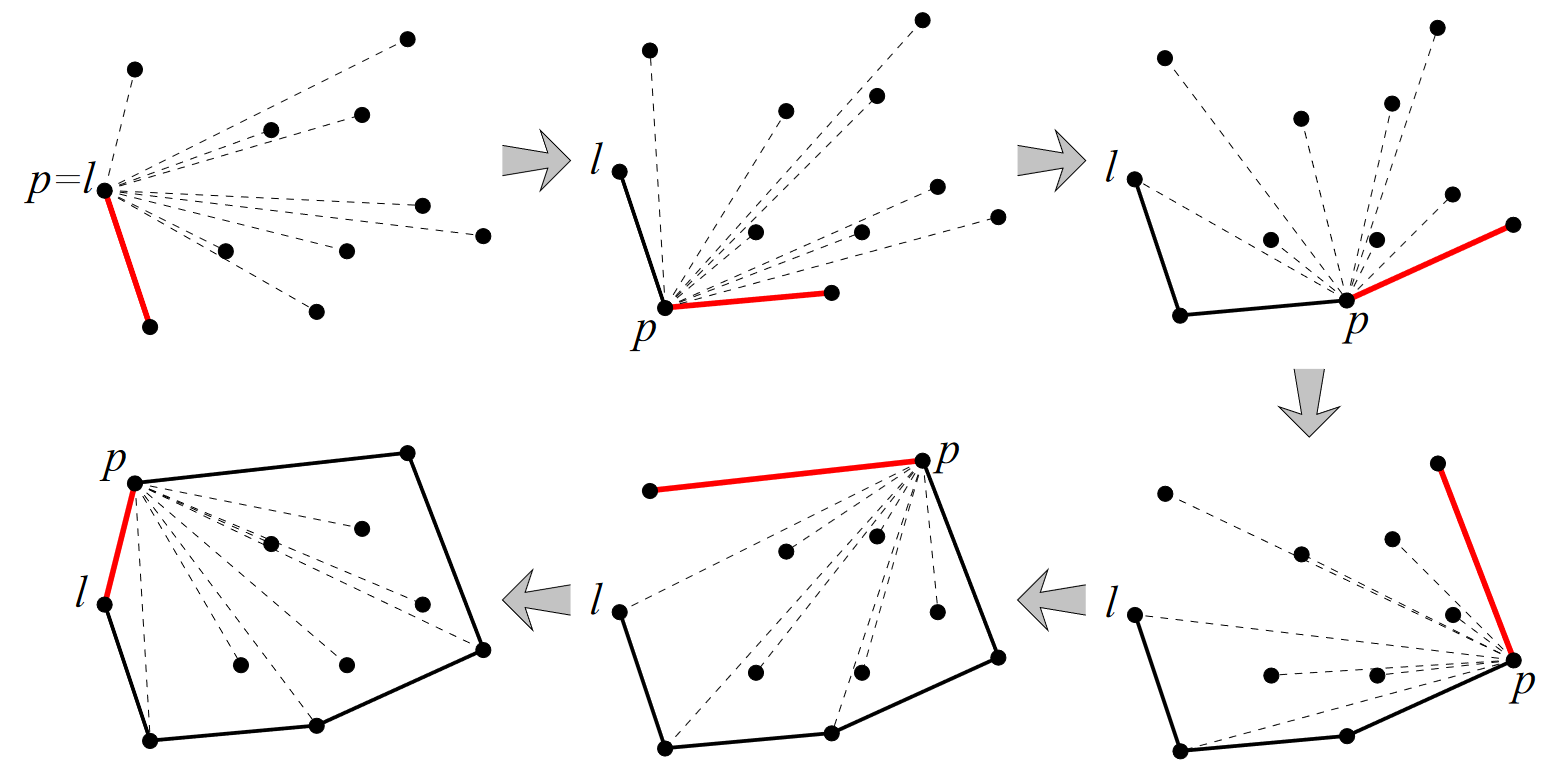
\includegraphics[width=0.7\textwidth]{jarvis/jarvis_visual.png}
\caption{\label{fig:jarvis_visual}Execution of the Jarvis’s Algorithm \cite{jeffe}}
\end{figure}

Given a convex hull vertex $p_i$ and its successor $p_{i+1}$, all the other points lie on the left of the line $p_i$ $p_{i+1}$. Then, starting with \textit{l} and continuing until we reach \textit{l} again, the algorithm finds each successive convex hull vertex. Each successor $p_{i+1}$ can be computed in linear time by performing a series of $O(n)$ comparisons.

\begin{codebox}
\Procname{$\proc{JarvisMarch}(S)$}
\li $hullPoint \gets$ index of leftmost point \Comment The leftmost point is guaranteed to be part of the $\proc{CH}(S)$
\li $i \gets 0$
\li \Repeat
\li     $CH[i] \gets S[hullPoint]$ \>\>\>\>\>\Comment CH will be the set of points which form the convex hull
\li     $endPoint \gets (hullPoint + 1)$ \% $|S| $ \>\>\>\>\>\>\>\Comment Make sure $hullPoint \neq endPoint$
\li     \For $j \gets 0$ \To $|S|$
        \Do
\li         \If $S[j]$ is on right of line from $CH[i]$ to $S[endPoint]$
\li         \Then
                $endPoint \gets j$ \>\>\>\>\>\Comment Found greater right turn, update endpoint
            \End
        \End
\li     $i \gets i+1$
\li     $hullPoint \gets endPoint$
\li \Until $hullPoint \isequal 0$
\li \Return CH
\end{codebox}

\subsubsection*{Algorithm analysis}
The pseudocode shows us that the worst-case running time is $O(n^2)$. However, Jarvis’s march is extremely fast if the convex hull has not so many vertices. We know that for each convex hull vertex, the algorithm spends $O(n)$ time to find the successor. Then, a better way to write the running time is $O(nh)$, where $h$ is the number of convex hull vertices. In the worst case we get a time complexity of $O(n^2)$ because $h = n$, but in the best case $h = 3$, and the algorithm only needs $O(n)$ time. Computational geometers call this an \textit{output-sensitive algorithm}. In computer science, an output-sensitive algorithm is an algorithm whose running time depends on the size of the output, instead of, or in addition to, the size of the input. \cite{wiki:1}

\subsubsection*{Implementation}

The following is a C++ implementation of the Jarvis's march algorithm. It stores the convex hull into a C++ vector which will contain the convex hull points in counter-clockwise order. 

\begin{listing}[H]
    \inputminted{cpp}{code/jarvismarch.cpp}
    \caption{C++ implementation of the Jarvis's algorithm}
\end{listing}

The code is totally inspired by the pseudocode, and the key parts are the usage of the functions \mintinline{c}{leftmost_point_index()} and \mintinline{c}{orientation()}. The first is used to compute, respectively, the index of the leftmost point. The second one is used to test if the points are in counter-clockwise order to check if a greater right turn has been found.

\newpage
\subsection{Graham's scan}

Just as in Jarvis's march, Graham's scan starts by finding the left-most point \textit{l} and it selects the bottom-most one if there is a tie. Then the algorithm does two main steps. The first one explicitly sorts the points in counter-clockwise order around the point \textit{l}. This can be done in $O(n\log{n})$ time with any sorting algorithm (quicksort, mergesort, etc...). The comparison between two points, let's say $a$ and $b$, is made by testing if the triple $lab$ is in counter-clockwise order or not. After sorting them, if you connect the points in counter-clockwise order you get a simple polygon with n points like the following one:

\begin{figure}[h]
\centering
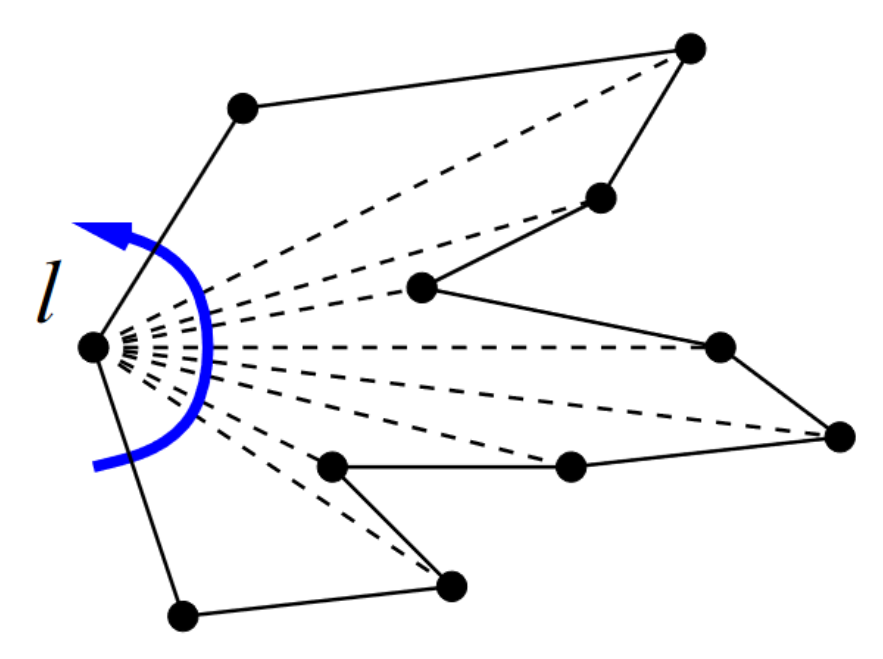
\includegraphics[width=0.2\textwidth]{graham/graham_visual_sorting.PNG}
\caption{\label{fig:graham_visual_sorting}The polygon after the sorting phase \cite{jeffe}}
\end{figure}

Now, the algorithm does the second and last step: it converts the polygon into the convex hull. To do that, for each point in the sorted sequence, it adds the current point to the convex hull. Then, it determines if the last 3 points in the convex-hull make a right turn. If they do, then the second-last point is not part of the convex hull, and it lies inside it, so it is removed from the convex-hull. The algorithm does it multiple times until the last 3 points do a left turn.

\begin{figure}[h]
\centering
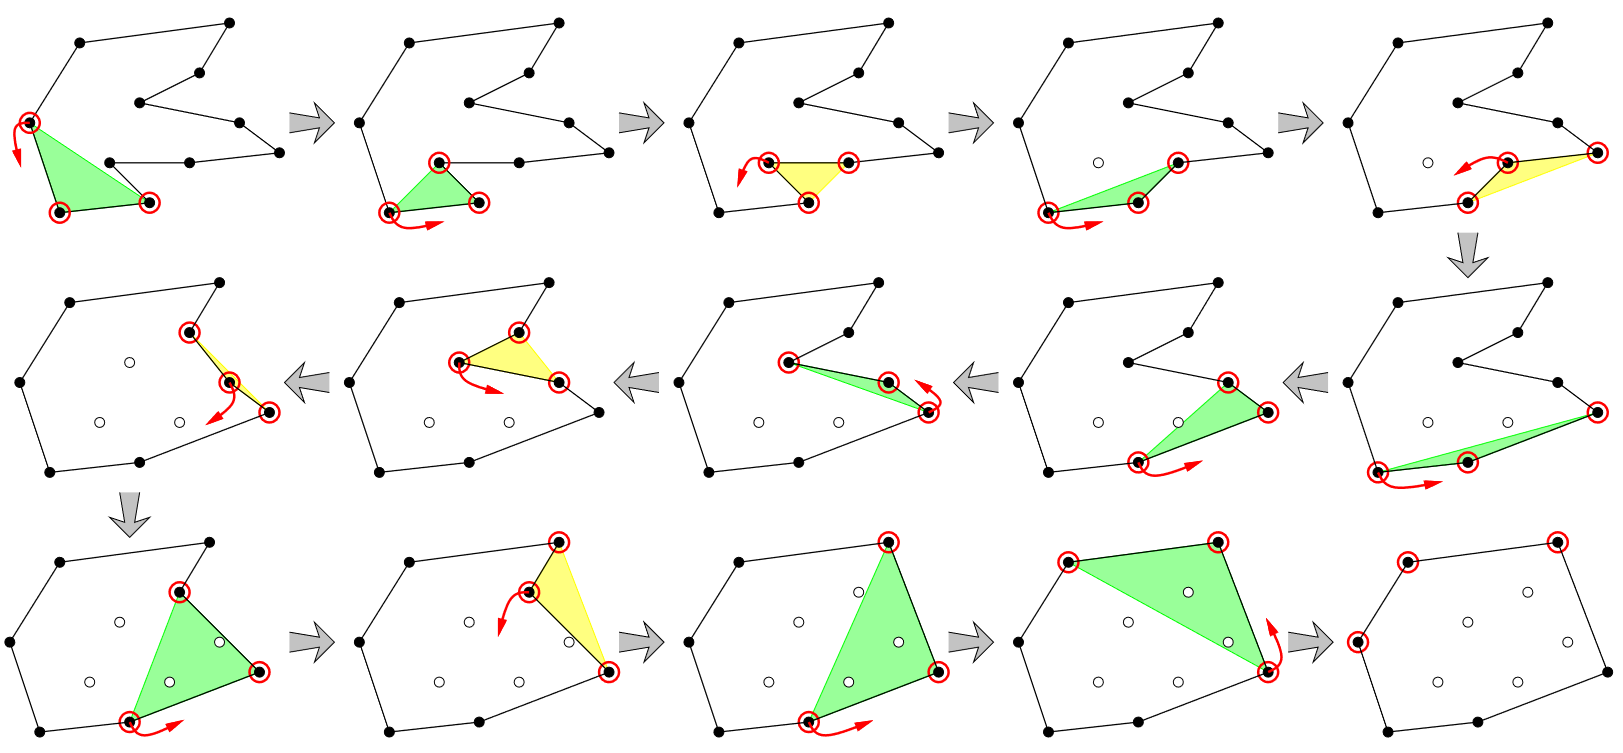
\includegraphics[width=0.9\textwidth]{graham/graham_visual.png}
\caption{\label{fig:graham_visual}Converting the polygon into the convex hull \cite{jeffe}}
\end{figure}

\begin{codebox}
\Procname{$\proc{GrahamScan}(S)$}
\li $p_0 \gets $ left-most point or bottom-most point if a tie
\li $\proc{SortCCW}(S, p_0)$ \Comment sort the points in counterclockwise order around $p_0$
\li $CH \gets $ empty stack
\li $\proc{Push}(p_0, CH)$
\li $\proc{Push}(p_1, CH)$
\li $\proc{Push}(p_2, CH)$
\li \For $i \gets 3$ \To $|S|$
    \Do
\li     \While not$ \proc{CCW}(\proc{NextToTop}(CH), \proc{Top}(CH), p_i)$
\li     \Do
            $\proc{Pop}(CH)$
        \End
\li     $\proc{Push}(p_i, CH)$
    \End
\li \Return $CH$

\end{codebox}

The function $\proc{NextToTop}()$ returns the item one entry below the top of the stack and the function $\proc{Top}()$ returns the topmost element. Both functions just return the point, without changing the stack. Given three points, $a$, $b$ and $c$, the predicate $\proc{CCW}()$ tests if $abc$ is in counter-clockwise order.

At the end of the algorithm, the stack contains the convex hull, where the points are oriented counter-clockwise and $p_0$ is the first point.

\subsubsection*{Algorithm analysis}
Sorting the points has time complexity $O(n\log{n})$, while the time complexity of the loop is $O(n)$ because each point is considered at most twice. Each point can appear only once as a second last point because in a "left turn" the algorithm advances to the next point, and in a "right turn" the point is removed. The overall time complexity is therefore $O(n\log{n})$, since the time to sort dominates the time to actually compute the convex hull.

\subsubsection*{Implementation}
The following is a C++ implementation of the Graham's scan algorithm.
\begin{listing}[H]
    \inputminted{cpp}{code/grahamscan.cpp}
    \caption{C++ implementation of the Graham's scan algorithm}
\end{listing}

While it is inspired by the pseudocode, this implementation doesn't use a stack but instead it uses a C++ vector from the C++ standard library. This approach makes easier to retrieve the point next to the top point. If the points in the convex hull are $k$ then the point next to the top is retrieved by just getting the $k-2$ element. 

After computing the leftmost point, Graham's scan needs to sort the points in counter-clockwise order from the leftmost point before computing the convex hull. It is important to pay attention at this step: the sorting phase checks the order between the given point and the leftmost one. Then, sorting together with the leftmost point will result into an unexpected behaviour. Because of that, the leftmost point is swapped with the point at the first position and the sorting is done from the second point to the last one. The function used to sort the points is the C++ \mintinline{c}{sort()} function from the C++ standard library. 

Because $Point$ is a custom class and the sorting is done in uncommon way, this implementation passes to the \mintinline{c}{sort()} function the function that should be used to compare the points. To keep the code shorter, the function is presented as a lambda function. The comparison is done between the two points and the leftmost one, but, if the three points are colinear, then the comparison is done by distance.

\newpage
\subsection{Quickhull}

Quickhull is a method of computing the convex hull that also works in n-dimensional space. It was invented in 1996 by Barber and Dobkin and it is a quick-sort like algorithm for convex hull, from which its name derives. It is essentially an iterative algorithm that adds individual points one point at a
time to an intermediate hull and uses a divide and conquer approach.

\begin{codebox}
\Procname{$\proc{QuickHull}(S)$}
\li $l \gets $ left-most point
\li $r \gets $ right-most point
\li $S1 \gets $ points in S that are on the right side of the oriented line from $l$ to $r$
\li $S2 \gets $ points in S that are on the right side of the oriented line from $r$ to $l$
\li $CH \gets $\{\} \Comment It will be the set of points which form the convex hull
\li 
\li $\proc{FindHull}(CH, S1, l, r)$
\li $\proc{FindHull}(CH, S2, r, l)$
\li
\li \Return $CH$
\end{codebox}

Initially, the algorithm finds the leftmost $l$ and rightmost $r$ points and it divides the points in two sets: the set of points that lie on the left of the segment $lr$ and the set of points that lie on the right.

\begin{figure}[h]
\centering
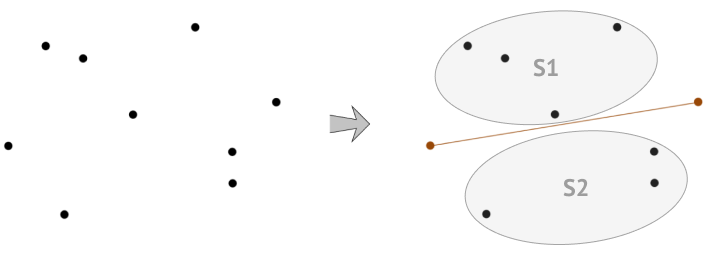
\includegraphics[width=0.5\textwidth]{quickhull/quickhull_visual_start.png}
\caption{\label{fig:quick_visual_start}Example of how the algorithm initially divides the set of points}
\end{figure}

Then, it calls the $\proc{FindHull}$ procedure for both sets. The procedure finds the farthest point from the segment and adds it to the convex hull. This produces a triangle made by the following three vertices: the farthest point $f$ and the two points $l$ and $r$ that made the segment.

\begin{figure}[h]
\centering
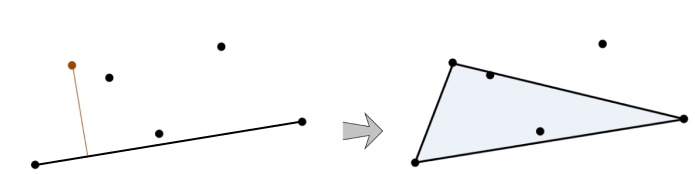
\includegraphics[width=0.5\textwidth]{quickhull/quickhull_visual_divide.png}
\caption{\label{fig:quick_visual_divide}Example of the triangle made by the farthest point and the given segment}
\end{figure}

At this point, the triangle partition the remaining points into three sets: the set of points that lie inside the triangle, the set of points that lie outside of the triangle which are in front of the segment $fr$, and the set of points that lie in front of the segment $lf$. The procedure, then, can ignore the points inside the triangle (because they are not part of the convex hull) and calls recursively on the other two sets. The following pseudocode summarizes the $\proc{FindHull}$ procedure: 

\begin{codebox}
\Procname{$\proc{FindHull}(CH, S_k, a, b)$}
\li \If $S_k$ is empty
\li \Then \Return \End
\li $f \gets $ farthest point in $Sk$ from segment $ab$
\li \Comment The points $a$, $b$, and $f$ partition the remaining points of $S_k$ into 3 subsets: $S0$, $S1$, and $S2$
\li $S1 \gets $ points in $S_k$ that are on the right side of the oriented line from $a$ to $f$
\li $S2 \gets $ points in $S_k$ that are on the right side of the oriented line from $f$ to $b$
\li
\li Add point $f$ to $CH$ at the location between $a$ and $b$
\li $\proc{FindHull}(CH, S1, a, f)$
\li $\proc{FindHull}(CH, S2, f, b)$
\end{codebox}

\subsubsection*{Algorithm analysis}
On average the algorithm works quite well, but it is slow in cases of high symmetry or when the points lie on the circumference of a circle. At the worst case the time complexity of the algorithm is $O(n^2)$ and at the average case it is $O(n\log{n})$.

\begin{figure}[h]
\centering
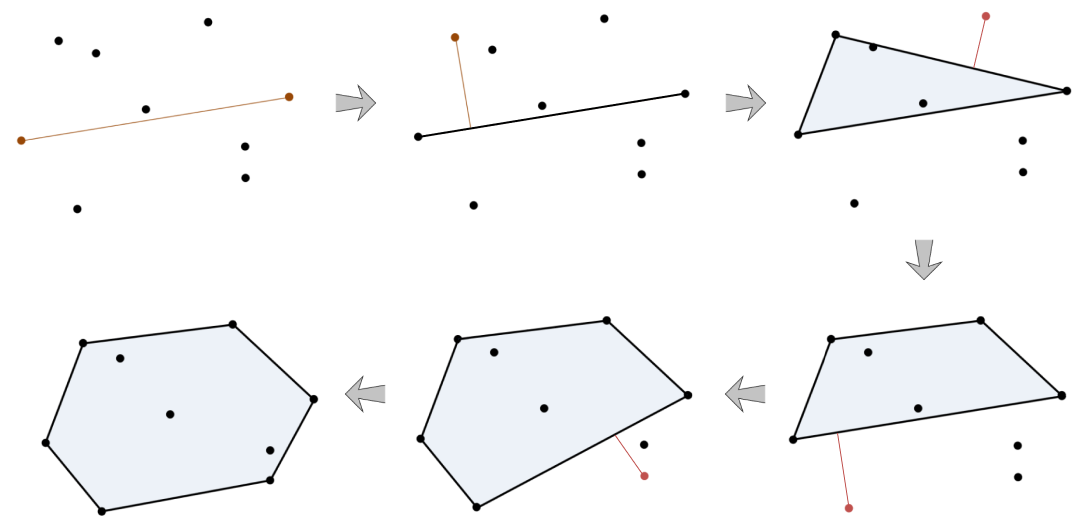
\includegraphics[width=0.7\textwidth]{quickhull/quickhull_visual.png}
\caption{\label{fig:quick_visual}Entire execution of the Quickhull algorithm}
\end{figure}

\subsubsection*{Implementation}
The following is a C++ implementation of the $\proc{QuickHull}$ procedure.
\begin{listing}[H]
    \inputminted[linenos]{cpp}{code/quickhull.cpp}
    \caption{C++ implementation of the $\proc{QuickHull}$ procedure}
\end{listing}

The implementation doesn't differ too much from the pseudocode. There are no particular cases to handle or particular functions to call. The only functions are the simple ones to retrieve the leftmost and the rightmost points and the function to get the orientation of three points. The key part of the implementation of the QuickHull algorithm is the \mintinline{c}{findhull()} function, which is the following:

\begin{listing}[H]
    \inputminted[linenos]{cpp}{code/findhull.cpp}
    \caption{C++ implementation of the $\proc{FindHull}$ procedure}
\end{listing}

The function \mintinline{c}{findhull()} takes as input the subset of points, a leftmost point $left$ and a rightmost point $right$. All the points in the input subset lie to the right of the line $left$-$right$.

The function initially computes the farthest point $far$ from the line $left$-$right$, then divides the points and does the two recursive calls. To stop the recursion, it is not enough to check if the input subset is empty: if all the remaining points lie exactly on top of the line $left$-$right$ (i.e, their distance from the line is zero) they must be discarded. So, after looking for the most distant point, if it is not found then the set is empty or all the subset of points lie above the line. When this happens, \mintinline{c}{findhull()} adds the leftmost point to the hull and the function stops without going further into the recursive calls. Because of that, during the execution, the hull is built in counter-clockwise order.

To split the set of points, the function iterates through all the points in the subset and for each point $p$ it checks if the line $left$-$far$-$p$ does a clockwise turn. If it does, then $p$ lies to the right of the line. Otherwise it checks if the $right$-$far$-$p$ does a counter-clockwise turn. It it does, then the point liew to the left of the line.

\newpage
\subsection{Divide and conquer}

Divide and conquer algorithms solve problems by dividing them into smaller instances, solving each instance recursively and merging the corresponding results to a complete solution. The following algorithm is a divide and conquer approach for the construction of the convex hull. It was invented by Preparata and Hong in 1977 \cite{preparata}.

\begin{codebox}
\Procname{$\proc{Preparata}(S)$}
\li $m \gets \left\lfloor n / 2 \right\rfloor$
\li $S1 \gets S[0..m]$
\li $S2 \gets S[m+1..n]$ 
\li $CH1 \gets \proc{Preparata}(S1)$
\li $CH2 \gets \proc{Preparata}(S2)$
\li $CH \gets $ merge $CH1$ and $CH2$
\li \Return $CH$
\end{codebox}

The algorithm requires that the set of points is sorted by x-coordinate, from the leftmost to the rightmost point. The algorithm recursively does the following steps. Given the point in the middle $p_m$, it partitions the set of points into the set of points on the left of $p_m$ (which contains $p_m$ as well) and the set of points on the right of $p_m$. Then, it recursively computes the convex hull of both sets and merges the resulting subhulls together by finding the tangents that connect the two hulls from above and below.

\begin{figure}[h]
\centering
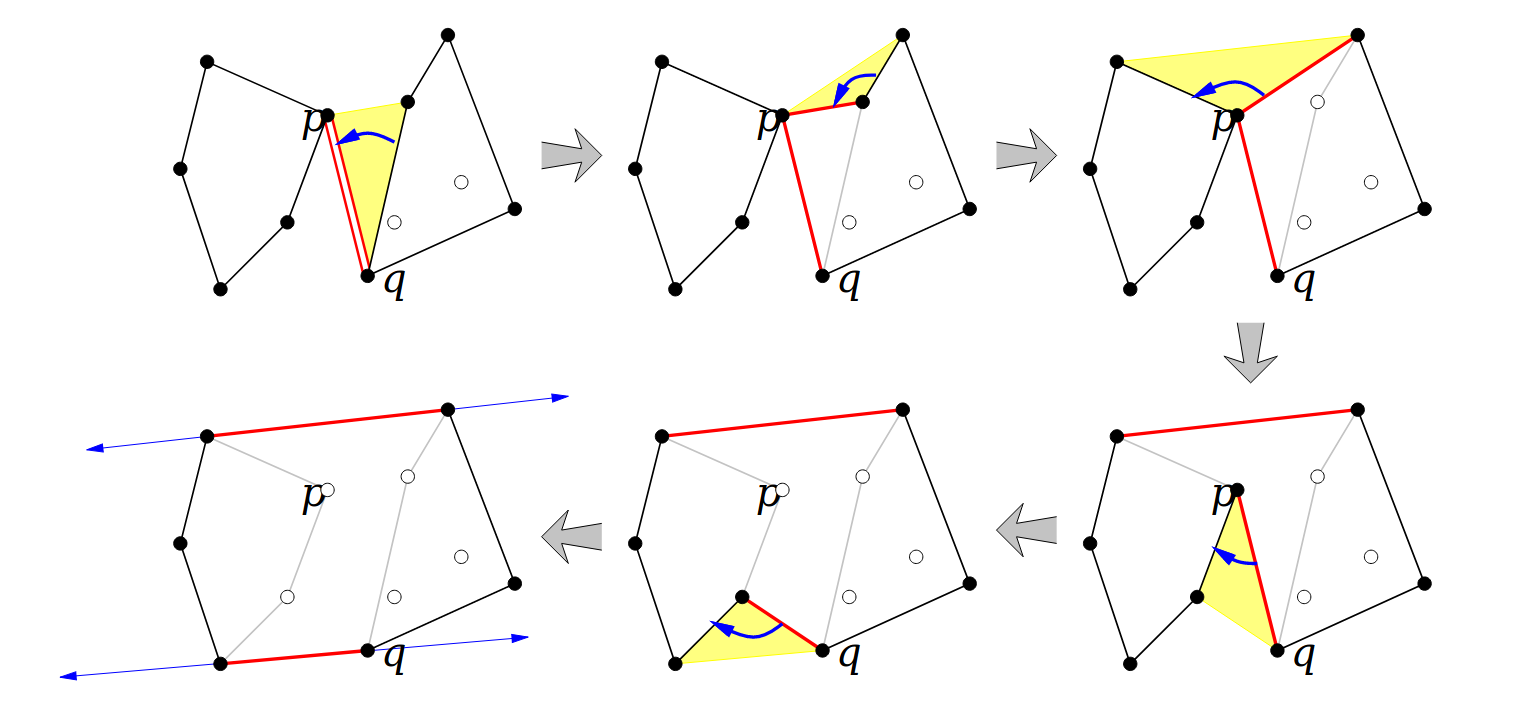
\includegraphics[width=0.9\textwidth]{preparata/preparata_visual_merge.png}
\caption{\label{fig:preparata_visual_merge}How the merge of two adjacent convex hulls is done \cite{jeffe}}
\end{figure}

To merge the subhulls, the algorithm creates two segments, called $bridges$, between the rightmost point of the left subhull and the leftmost point of the right subhull. As long as there is a clockwise turn at either endpoint of either bridge, the point is removed and its two neighbors became connected. As soon as the turns at both endpoints of both bridges are counter-clockwise, the algorithm stops. Note that, after merging the subhulls, the bridges lie on the upper and lower common tangent lines of the two subhulls.

\subsubsection*{Algorithm analysis}
It is clear that this algorithm resembles to QuickSort. The running time is given by the recurrence $T(n) = O(n) + T(k) + T(n-k)$, just like QuickSort, where $k$ is the number of points to the right of the middle point $p_m$. Just like QuickSort, a deterministic approach to chose $p_m$ will result into a $O(n^2)$ time complexity at worst case. If $p_m$ is chosen randomly, then the running time is expected to be $O(n\log{n})$. Note that there are input where this algorithm is not practical.

\subsubsection*{Implementation}
The implementation of this algorithm follows the typical divide and conquer approach. It uses the function \mintinline{c}{ch_three_points()} which computes the convex hull of three points.
\begin{listing}[H]
    \inputminted[linenos]{cpp}{code/preparata.cpp}
    \caption{C++ implementation of the $\proc{Preparata}$ procedure}
\end{listing}

The important phase of the algorithm is of course the merging phase, which is implemented like the following:
\begin{listing}[H]
    \inputminted[linenos]{cpp}{code/preparata_merge.cpp}
    \caption{Merging two subhulls into one}
\end{listing}

The function to compute the upper bridge is given below. The one for computing the lower bridge is the same but it is specular. To find the upper bridge, the algorithm starts with two points, one from each subhull, and then iteratively goes clockwise or counter-clockwise from the first or the second points until the line that connects the two points is the upper tangent line of the two subhulls. 
\begin{listing}[H]
    \inputminted[linenos]{cpp}{code/preparata_upper_bridge.cpp}
    \caption{Computing the upper bridge}
\end{listing}

\newpage
\subsection{Monotone chain}

The Andrew's Monotone chain method is a simple way to compute the convex hull of a set of points in 2-dimensions. First thing first it sorts the points by x-coordinate, and in case of a tie, by y-coordinate. After the sorting phase, it constructs the lower hull by starting from the leftmost point and trying to go counter-clockwise as much as possible until it reaches the rightmost point. Then, it constructs the upper hull going back from the rightmost point to the leftmost and trying to go counter-clockwise as much as possible. The algorithm's pseudocode is given below.

\begin{codebox}
\Procname{$\proc{MonotoneChain}(S)$}
\li $\proc{Sort}(S)$ \Comment Sort the points by x-coordinate or by y-coordinate in case of a tie
\li $CH \gets $\{$S[0]$\} \Comment It will be the set of points which form the convex hull
\li $i \gets 0$
\li \While $i < |S|$
    \Do
\li     \If $|CH| >= 2$ and $ \proc{CW}(\proc{NextToTop}(CH), \proc{Top}(CH), S[i])$
        \Then
\li         $\proc{Pop}(CH)$ \Comment Found clockwise turn, update the hull
\li        \Else
\li            $\proc{Push}(CH, S[i])$
\li            $i \gets i+1$
        \End
    \End
\li
\li $i \gets |S|-2$
\li \While $i >= 0$
    \Do
\li     \If $|CH| >= 2$ and $\proc{CW}(\proc{NextToTop}(CH), \proc{Top}(CH), S[i])$
        \Then
\li         $\proc{Pop}(CH)$ \Comment Found clockwise turn, update the hull
\li     \Else
\li         $\proc{Push}(CH, S[i])$
\li         $i \gets i-1$
        \End
    \End
\li
\li \Return $CH$
\end{codebox}

The following figure gives a visualization of how the algorithm constructs the upper hull. During the iteration it keeps track of the intermediate convex hull by keeping the sequence of the previous scanned points that have counter-clockwise order. It starts from the leftmost point and scans the sorted points until it reaches the rightmost point. For each point, if the last point in the intermediate convex hull and the current point are in clockwise order, then the algorithm removes the last point from the intermediate convex hull and evaluates again the current point until it is in counter-clockwise order with the last point of the intermediate convex hull.

\begin{figure}[h]
\centering
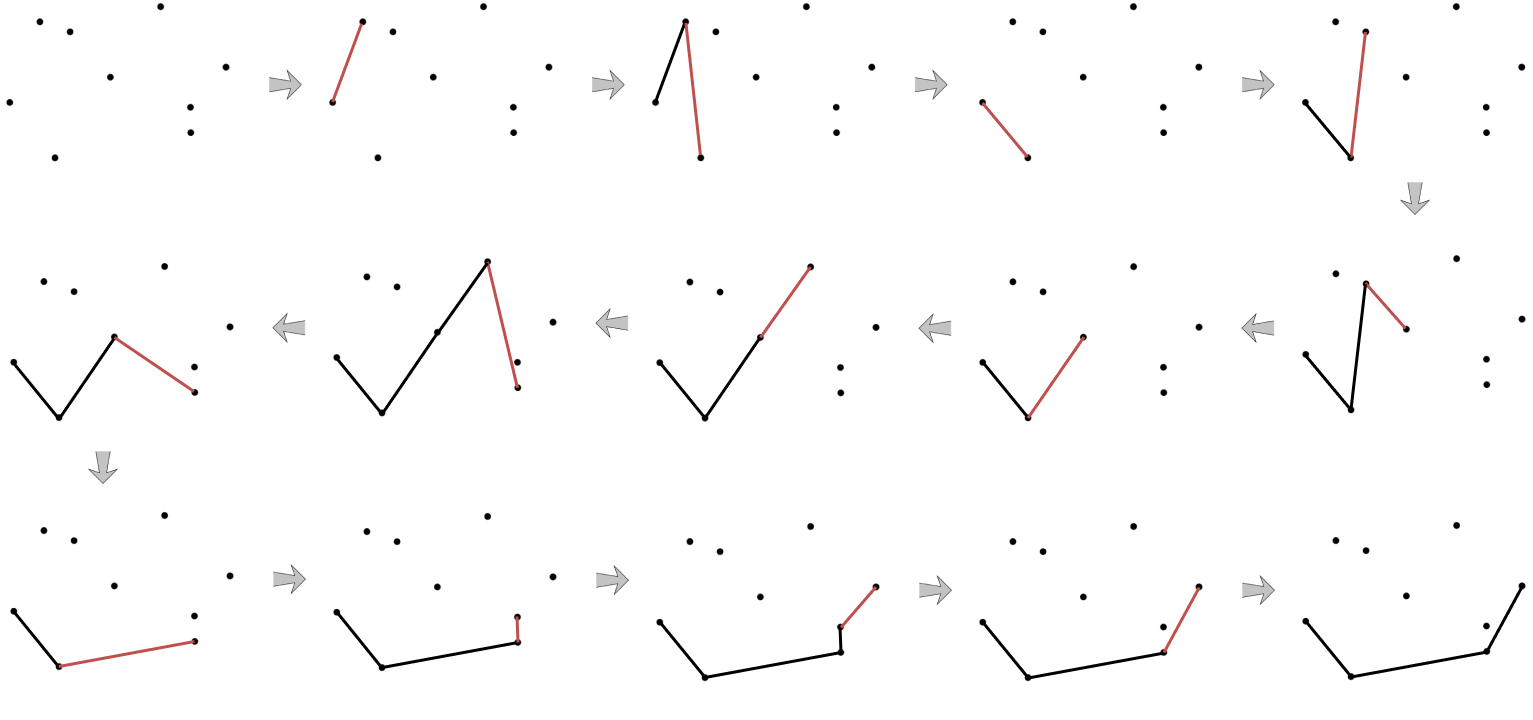
\includegraphics[width=0.9\textwidth]{monotone/monotone_visual.png}
\caption{\label{fig:monotone_visual}Example execution of how the Monotone chain algorithm constructs the upper hull}
\end{figure}

Then, the algorithm applies the same approach to construct the lower hull by scanning the points from the rightmost to the leftmost and testing if the points have a counter-clockwise order.

\subsubsection*{Algorithm analysis}
The construction of the upper and lower hulls of the points have time complexity of $O(n)$ time, because the algorithm linearly scans each point.
The overall time complexity is therefore $O(n\log{n})$, since the time to sort dominates the time to actually compute the convex hull.

\subsubsection*{Implementation}
\begin{listing}[H]
    \inputminted[linenos]{cpp}{code/monotonechain.cpp}
    \caption{C++ implementation of Monotone Chain algorithm}
\end{listing}

\newpage
\subsection{Incremental convex hull algorithm}

The Incremental convex hull algorithm computes the convex hull by iteratively adding points \cite{incremental}. The algorithm iterates through all the points and, for each point, it tests if the point is inside or outside the hull. If a point is already in the hull then it is ignored, otherwise it is added to the hull. If a point is outside of the hull then it can "see" a certain amount of other points in the hull. Doesn't matter how many of them the point can see, there will always be two points, called \textit{transition points}, that are the last two points that the point can see (after them, all the other points cannot be seen by the current point). So the algorithm removes the other ones from the hull and the point is added to the hull between the two transition points.

\begin{figure}[h]
\centering
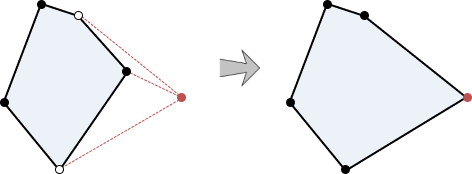
\includegraphics[width=0.4\textwidth]{incremental/incremental_visual_visible.png}
\caption{\label{fig:incremental_visual_visible}Here the red point can see three points. The transition points are the white points, because after them there are only points not visible from the red point. The transition points should remain into the hull, while the other non-transition points that are visible from the red point should be removed from the hull.}
\end{figure}

\begin{codebox}
\Procname{$\proc{IncrementalCH}(S)$}
\li $\proc{Sort}(S)$ \Comment Sort the points from the leftmost to the rightmost (i.e, by x-coordinate)
\li $CH \gets $\{$S[0], S[1], S[2]$\}
\li \For $i \gets 3$ \To $|S|$
    \Do
\li     $t_{1}, t_{2} \gets \proc{TransitionPoints}(CH, S[i])$
\li     $\proc{RemoveBetween}(CH, t_{1}, t_{2})$ \Comment Remove the points between the transition points
\li     $\proc{AddBetween}(CH, S[i], t_{1}, t_{2})$ \Comment Add the current point between the transition points
    \End
\li \Return $CH$
\end{codebox}

To compute if a point is outside or inside the hull, the algorithm should compare the point with each point in the hull. This will take linear time, so the overall time complexity of the algorithm will become $O(n^2)$. However, the Incremental convex hull algorithm uses a better approach, and it can compute if a point lies inside or outside the hull faster. To do that, the algorithm first sorts the points by x-coordinate. Since the points are sorted, each new point considered must see the previous added point. Any vertex traversed to find the transition point is removed.

\begin{figure}[h]
\centering
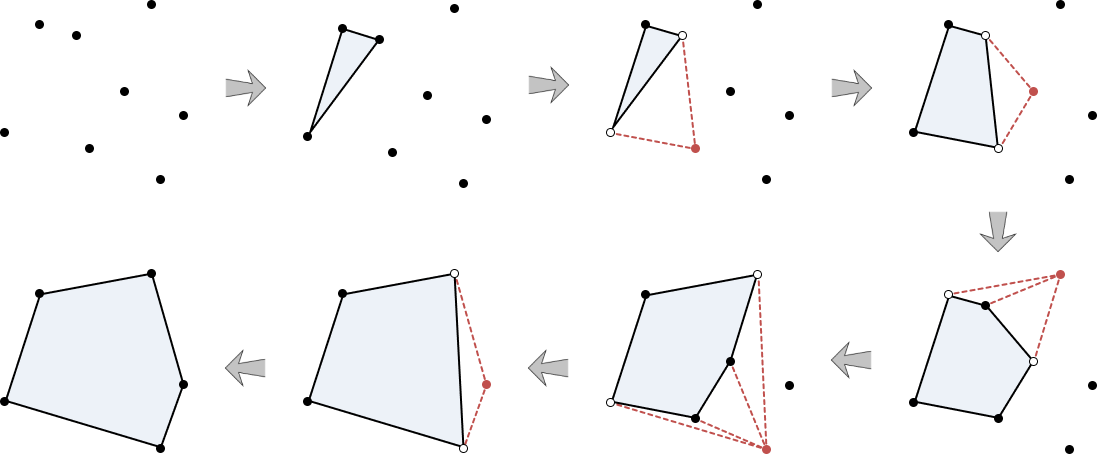
\includegraphics[width=0.7\textwidth]{incremental/incremental_visual.png}
\caption{\label{fig:incremental_visual}Execution of the incremental convex hull algorithm}
\end{figure}

\subsubsection*{Algorithm analysis}
By sorting the points it is possible to compute the transition points in constant time. So, computing the convex hull takes $O(n)$ time. The overall time complexity is therefore $O(n\log{n})$, since the time to sort dominates the time to actually compute the convex hull.

\subsubsection*{Implementation}
A good implementation of the Incremental convex hull algorithm has to efficiently manage the convex hull points because it is needed to add/remove points between two transition positions. The STL C++ vector is not suitable because removing points from two positions will also need to shift to the left some points from the farthest position. An approach with a double linkedlist can be useful but it will be sensible to cache misses and should be avoided as well. The following is a C++ implementation of the algorihtm and uses a different and more efficient approach.

\begin{listing}[H]
    \inputminted[linenos]{cpp}{code/incremental.cpp}
    \caption{C++ implementation of the Incremental convex hull algorithm}
\end{listing}

This implementation uses a matrix of two columns and $n$ rows, where $n$ is the number of the given points. The $i-th$ row stores the indexes of the successor and predecessor of the $i-th$. In other words, it is like an adjacency matrix of a graph in which the nodes are the convex hull points and each node has two edges. With this approach, removing and adding points between the two transition points is very efficient, it has linear time complexity, it does not need to shift any points and it is not sensible to cache misses.

\newpage
\subsection{Kirkpatrick–Seidel algorithm}

The Kirkpatrick–Seidel algorithm, named after its inventors, David G. Kirkpatrick and Raimund Seidel, is a divide and conquer algorithm \cite{kirkseidel}. Like the monotone chain method, the Kirkpatrick–Seidel algorithm computes the upper-hull and the lower-hull and then merges them. The algorithm to compute the upper-hull is given below. The lower-hull can be computed in a similar manner and is omitted from further discussion. 

Compared to the divide and conquer algorithm by Preparata, the Kirkpatrick–Seidel algorithm reverses the order of the dividing and merging steps. Instead of dividing first and merging after, the algorithm first merges the upper subhulls by computing the upper bridge that connects the two sub hulls and then divides the points. Because of that, this algorithm is also called by its authors as \textit{Marriage Before Conquest}.

\begin{codebox}
\Procname{$\proc{MBCUpperHull}(S)$}
\li $med \gets$ the index of the median of x-coordinates of points in $S$
\li $L \gets S[0..med]$
\li $R \gets S[med+1..|S|]$
\li $p, q \gets $ upper bridge of L and R, $p\in L$ and $q\in R$
\li $L' \gets $\{ $l \in L \mid x(l) \leq x(p)$ \}
\li $R' \gets $\{ $r \in R \mid x(r) \geq x(q)$ \}
\li $LUH \gets \proc{MBCUpperHull(L')}$
\li $RUH \gets \proc{MBCUpperHull(R')}$
\li \Return the concatenation $LUH$, $pq$, $RUH$
\end{codebox}

As per the definition of a convex hull, all the points below the upper bridge can not be a part of the upper hull. Dividing the points after computing the bridge allows to efficiently evaluate only the points that can possibly be part of the hull. In the case of divide and conquer algorithm by Preparata, finding bridges constitute the “merge” step of the algorithm. In this algorithm, finding bridges are the primary algorithmic step.

The algorithm works by finding the median x-coordinate and then finding the bridge. The points in the bridge are added to the hull. The remaining points are split into two sets: the set of points to the left of the bridge, and the set of points to the right. The algorithm is called recursively on each subset.

\subsubsection*{Finding the Bridge}
Computing the bridge can be done in $O(n)$ time thanks to a \textit{Prune and Search} technique which allows to eliminate a good many of the points that do not define the upper bridge \cite{pruneandsearch}. More formally, the bridge is a line $t$ that passes through one point from the left subset and one point from the right subset, such that none of the given points lie above $t$.

The set of points is partitioned into two subsets by the vertical line defined by the median $x_{m}$. We can have an upper supporting line $L$ which is tangent to the set of points at a point $p_t$. If an upper supporting line contains points to the left of $x_{m}$ and also points to the right, then the supporting line contains the bridge. Otherwise, we have the following observations. Given any two points $r$ and $s$ from the set of points, such that $r$ is to the left of $s$
\begin{itemize}
  \item if $x(p_{t}) < x_{m}$ and $slope(\overline{\rm rs}) \geq slope(L)$, then the bridge doesn't pass through $r$
  \item if $x(p_{t}) \geq x_{m}$ and $slope(\overline{\rm rs}) < slope(L)$, then the bridge doesn't pass through $s$
\end{itemize}

\begin{figure}[h]
    \centering
    \begin{subfigure}[b]{.22\linewidth}
        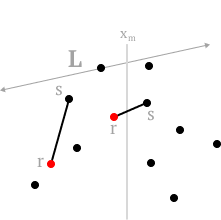
\includegraphics[width=\textwidth]{kirk/kirk_visual_supp_line_a.png}
        \caption{\label{fig:kirk_visual_supp_line_a}}
    \end{subfigure}
    \hspace{14mm}
    \begin{subfigure}[b]{.22\linewidth}
        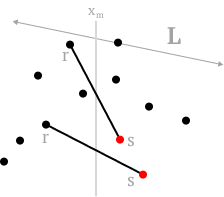
\includegraphics[width=\textwidth]{kirk/kirk_visual_supp_line_b.png}
        \caption{\label{fig:kirk_visual_supp_line_b}}
    \end{subfigure}
    
    \caption{\label{fig:kirk_visual_supp_line}Example of the previous observations. The red points can be removed.}
\end{figure}

To prove our observations, let's just think about the first case for now, when $p_t$ has x-coordinate $< x_{m}$. In that case $L$ doesn't pass through any point to the right of the median, and it passes through $p_t$, which is to the left. Because of that, the slope of the bridge must be lower than the slope of $L$. So, if $slope(\overline{\rm rs}) < slope(L)$ (Figure \ref{fig:kirk_visual_supp_line_b}), then the bridge cannot pass through $r$ because if it does then it will pass below $s$ and it cannot be possible by the definition of bridge. 

Similarly, when $L$ contains only points to the right of the median, which means that $p_t$ has x-coordinate $\geq x_{m}$, then the slope of the bridge must be greater than the slope of $L$. So, if $slope(\overline{\rm rs}) \geq slope(L)$ (Figure \ref{fig:kirk_visual_supp_line_a}) then the point $s$ is not part of the bridge, otherwise it will imply that the bridge passes below $r$ but it is a contradiction so the point $s$ cannot be part of the bridge.

\begin{figure}[h]
\centering
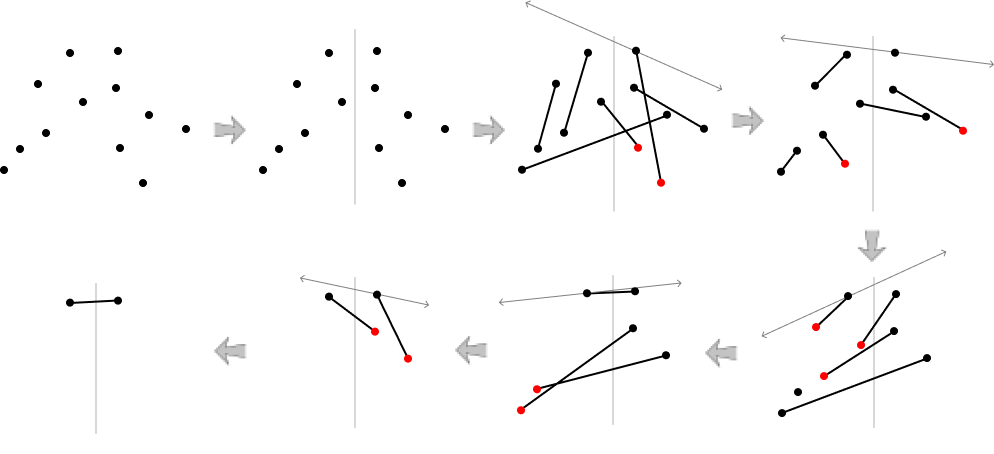
\includegraphics[width=0.85\textwidth]{kirk/kirk_visual_bridge.png}
\caption{\label{fig:kirk_visual_bridge}Computing the bridge with the \textit{Prune and Search} technique}
\end{figure}

These remarks suggest how the \textit{Prune and Search} method works. The algorithm randomly pairs the given points and finds the median slope $\alpha$ of the $\frac{n}{2}$ segments defined by those pairs. Then it computes a line $L$ of slope $\alpha$ that passes through a point $p_t$ such that it is an upper supporting line for the set of points. Because $\alpha$ is the median slope, then half pairs have slope less than $\alpha$, and half have greater slope. To prune the set of possible bridge points, the algorithm iterates through all the pairs $rs$ and removes $r$ if $x(p_t) \geq x_m$ and $slope(\overline{\rm rs}) < \alpha$ or removes $s$ if $x(p_t) < x_m$ and $slope(\overline{\rm rs}) > \alpha$. The Figure \ref{fig:kirk_visual_bridge} shows an example of how the bridge is computed by the \textit{Prune and Search} technique. Therefore, after every iteration $\frac{1}{4}$ of the remaining points are removed from consideration as bridge points \cite{kirk_tufts}.

\subsubsection*{Algorithm analysis}
Given a set of $n$ points, the Kirkpatrick–Seidel algorithm computes the convex hull in $O(n\log{h})$ time, where h is the number of convex hull vertices. Thus, the algorithm is output-sensitive: as said before, its running time depends on both the input size and the output size. 

\subsubsection*{Implementation}

The important part of the implementation of the Kirkpatrick–Seidel algorithm is how it computes the upper bridge with \textit{Prune and Search} technique. Initially the algorithm pairs the points and this is straightforward and can be done by iterating through all the points. If the number of points is odd then the last point is ignored.  During the iteration it is possible to compute the slope of each segment and to compute the average later. 

Then, it is needed to find a supporting line for the set of points which passes through a point $p_t$. Because we know the slope of the line, it is possible to calculate the equation of the line passing through a point. From the equation, it is also possible to compute where the line intersects the y-axis. The point $p_t$ is that point such that when the line passes through it, it intersects the y-axis higher compared when the same line passes through the other points. This approach to compute $p_t$ can be done by iterating through all the points, computing the equation of the line and the intersection with the y-axis. 

The C++ implementation of how the Kirkpatrick–Seidel algorithm computes the upper bridge is given below. The approach for the lower bridge is the same but it is simmetrical.

\begin{listing}[H]
    \inputminted[linenos]{cpp}{code/kirk.cpp}
    \caption{C++ code for finding the upper bridge}
\end{listing}

\newpage
\subsection{Chan's algorithm}

The Chan's algorithm, named after Timothy M. Chan, who published it in 1993, is an optimal output-sensitive algorithm to compute the convex hull of a set of points, in 2 or 3-dimensional space. It is a combination of divide and conquer and gift wrapping.

The algorithm works by dividing the $n$ points into $n/m$ subsets, each of size at most $m$, and computing the convex hull of each subset using Graham's scan (for example).

\begin{figure}[h]
\centering
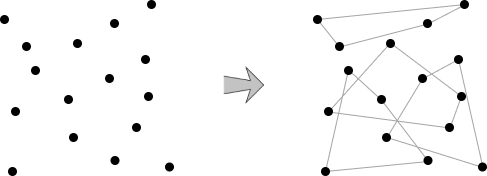
\includegraphics[width=0.5\textwidth]{chan/chan_visual_subhulls.png}
\caption{\label{fig:chan_visual_subhulls}Example of subhulls. Here the set of points is divided into 4 subsets. Note that the subset can intersect each other or not. Figure inspired by \cite{jeffe}}
\end{figure}

After computing the $n/m$ subhulls, Chan's algorithm applies Jarvis's march (gift wrapping) algorithm: starting with the rightmost point $l$, the algorithm successively finds the convex hull point that follows the last computed convex hull point in a counter-clockwise order until it returns to $l$ again.

\begin{figure}[h]
\centering
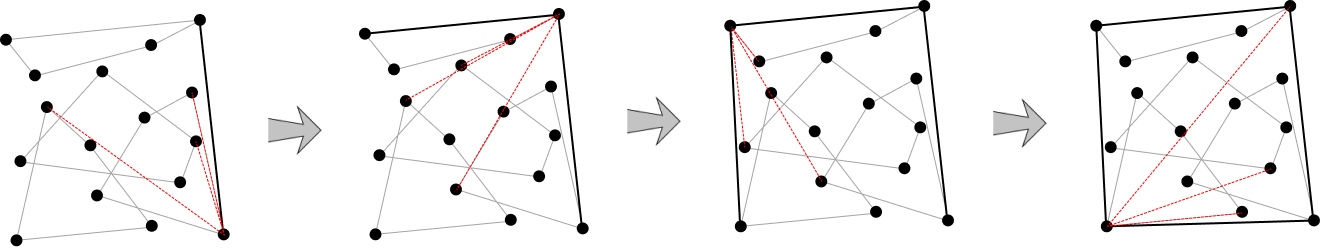
\includegraphics[width=0.9\textwidth]{chan/chan_visual_wrapping.png}
\caption{\label{fig:chan_visual_wrapping}Wrapping the subhulls. The dashed red lines are the other candidates other than the selected one. Figure inspired by \cite{jeffe}}
\end{figure}

Timothy Chan in his paper suggests a binary search approach to be used by the Jarvis's march algorithm to efficiently wrap all the subhulls \cite{chan}. At each step, given the last computed convex hull point $p_i$, Jarvis's march needs to find a point $p_{i+1}$ that follows $p_i$ in the convex hull in counter-clockwise order. More formally, it needs to find a point $p_{i+1}$ such that all other points are to the right of the line $\overline{\rm p_{i}p_{i+1}}$. The point $p_{i+1}$ is part of one of the $n/m$ subhulls, so the algorithm has $n/m$ possible candidates, one for each subhull. The $m$ points in a subhull are sorted in counter-clockwise order and this allows to use binary search to compute the subhull's candidate point in logaritmic time. At this point, the algorithm can efficiently determine $p_{i+1}$ with the Jarvis's march algorithm, by only considering the $n/m$ possible candidates instead of the whole set of points.

\begin{codebox}
\Procname{$\proc{ChanAlgorithm}(S, m, H)$}
\li $P_i , ... , P_{n/m} \gets$ partition S into $n/m$ subsets
\li \For $i \gets 0$ \To $n/m$
    \Do
\li $CH_i \gets \proc{GrahamScan}(P_i)$ \Comment the vertices are stored in an array in ccw order
    \End
\li $p_0 \gets (0, -\infty)$
\li $p_1 \gets$ rightmost point of $S$
\li \For $k \gets 1$ \To $H$
    \Do
\li     \For $i \gets 0$ \To $\left\lceil n / m \right\rceil$
        \Do
\li         compute $q_i \in P_i$ that maximizes the angle $\overline{\rm p_{k-1}p_{k}q_i}$ by binary searching on the\\
        \>\>points in $P_i$
        \End
\li     $p_{k+1} \gets $ the point $q$ from $\{q_{1}, ..., q_{\left\lceil n / m \right\rceil}\}$ that maximizes the angle $\overline{\rm p_{k-1}p_{k}q}$
\li     \If $p_{k+1} = p_1$
        \Then
\li          \Return $\{p_1, ..., p_k\}$
        \End
    \End
\li \Return $incomplete$
\end{codebox}

\subsubsection*{Guessing the value of \textit{m}}

Since the value of $h$ is not known in advance, the idea is to make multiple passes of the algorithm with increasing values of $m$. It is important to increase the value properly: if $m$ increases too slowly, the number of iterations may be large; if it increases too quickly, the algorithm terminates successfully but $m$ may be much larger than $h$ and it will produce a time complexity much higher than $O(nlogh)$. One possible strategy is to square the value of $m$ starting from a value of 2. With this squaring strategy, $O(loglogh)$ iterations are made. The following pseudocode shows the described approach. 

\begin{codebox}
\Procname{$\proc{ChanAlgorithm}(S)$}
\li \For $t \gets 1, 2, ...$
    \Do
\li     $L \gets \proc{ChanAlgorithm}(S, m, H)$, where $m = H = min\{2^{2^t}, n\}$
\li     \If $L \neq incomplete$
        \Then
\li         \Return $L$
        \End
    \End
\end{codebox}

\subsubsection*{Algorithm analysis}

The algorithm can be subdivided into two main phases. The first phase, which consists of partitioning the set of points and computing each subhull, takes $O(\frac{n}{m}m\log{m}) \gets O(n\log{m})$ time, because each subset has $m$ points, the subhull is computed in $O(m\log{m})$ time and we have $n/m$ subsets.

The second and last phase consists of wrapping the subhulls with the Jarvis's march algorithm and a binary search approach. Because of the way the algorithm works, Jarvis's march computes the convex hull in $O(h)$ iterations, where $h$ is the number of convex hull points. For each iteration, to find the the next convex hull point, the algorithm binary searches each subhull to find $n/m$ possible candidates. This search takes $O(\frac{n}{m}\log{m})$ time, because binary searching in one subhull costs time $O(\log{m})$ and we have $n/m$ subhulls. So, the second phase takes $O(\frac{n}{m}h\log{m})$. If $m$ is close to $h$ then the overall time complexity of Chan's algorithm is equivalent to $O(n\log{h})$.

To guess the value of $m$, at each iteration the algorithm squares the value of $m$. The number of iterations is $O(\left\lceil \log{\log{h}} \right\rceil)$, because it stops when the value of $H$ reaches or exceeds $h$. An iteration $t$ has a cost of $O(n\log{H}) \gets O(n2^t)$ time (using base-2 logarithms). Therefore, the total running time of the algorithm is $O(\sum_{t=1}^{\left\lceil \log{\log{h}} \right\rceil} n2^t) \gets O(n2^{\left\lceil \log{\log{h}} \right\rceil + 1}) \gets O(n\log{h})$.

\subsubsection*{Implementation}
Before looking at how to implement the Chan's algorithm, let's have a look to how the simple binary search works. The c++ implementation is given below:
\begin{listing}[H]
    \inputminted[linenos]{cpp}{code/chan_binary_search.cpp}
    \caption{Binary search the next candidate from the given subhull}
\end{listing}
Given the subhull and the last added point into the convex hull, the function binary searches for the next possible candidate. The points in the subhull are sorted in counter-clockwise order. So, it starts from the first element and goes forward when it is needed to go counter-clockwise otherwise it goes backward. Instead of iterating through all the points, the algorithm goes forward/backward a value multiple of two which is smaller after each iteration until if finds the best next candidate.

Then, the C++ implementation of the Chan's algorithm is the following. It calls the Graham Scan function to compute the subhulls and it uses the \mintinline{c}{next_candidate()} to binary search the next possible candidate from each subhull.

\begin{listing}[H]
    \inputminted[linenos]{cpp}{code/chan.cpp}
    \caption{C++ implementation of Chan's algorithm}
\end{listing}

It is important to note that, the jarvis phase does not differ too much from the real Jarvis's march algorithm, because the approach is still the same. Thanks to the binary search phase, the number of candidates is lower for each iteration and the algorithm runs efficiently.

\newpage
\section{Higher dimensions}

As seen before, in 2 dimensions the convex hull is a convex polygon. A convex polygon is the 2-dimensional example of a polytope, which is a geometric object with flat sides (called faces). In any number of dimensions, the convex hull is a convex polytope. In 3 dimensions, the convex hull is a convex polyhedron, which is a 3-dimensional example of a polytope.

Some algorithms that can compute the convex hull of a set of points in 2-dimensional space can also be extended to work on 3 or higher dimensions.The following are the algorithms that, with the right approach, can compute the convex hull in higher dimensions:

\begin{itemize}
  \item Incremental convex hull, which is slower but preferred in practice
  \item QuickHull, which is slower but preferred in practice for dimensions higher than 3
  \item Divide and conquer, which is elegant but difficult to implement
  \item Jarvis's march, which is used by the divide and conquer algorithm
  \item Chan's algorithm, that is preferred in 3 dimensions
\end{itemize}

\subsection{Visibility}
Like in the 2-dimensional case, in higher dimensions there is also the need to understand the concept of visibility: Given some points, what are the points that can "see" a given face $f$ of the polytope. For simplicity we can think about a 3-dimensional polytope, the polyhedron. To answer this question we can take the plane $h_f$ that expands by the face $f$ and, if the segment from $p$ to $f$ doesn't pass through any other face of the polytope, then the point is visible from the face. Otherwise, if the segment passes through another face, the point is not visible from the face.

\begin{figure}[h]
\centering
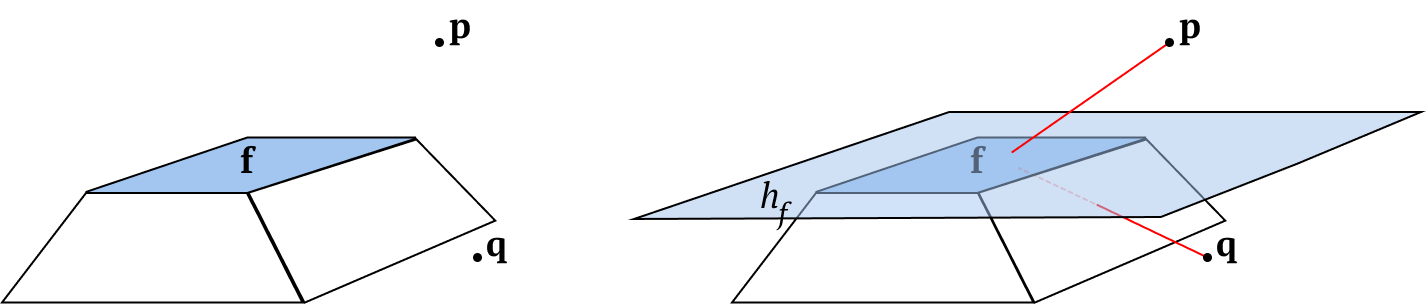
\includegraphics[width=0.55\textwidth]{higher_dim/threedim_visibility.png}
\caption{\label{fig:higher_dimensions_visibility} The face $f$ is visible from the point $p$ but not from the point $q$: the red segment from the face to $p$ does not pass through the polyhedron; the segment from the face to $q$ passes through another face of the polyhedron. This figure is inspired by the book \cite{computgeombook}.}
\end{figure}

Given a polytope and a point $r$, we can then know the set of faces that are visible from the point, and the set of the faces that cannot be seen by the point. To do this we can draw a ray from the point to any other point of the convex hull. For some points, the ray will go inside the polytope but for some other points the ray will just touch the point without going inside the polytope. Such points are the last points that can the point can see. If we look at the projection to a plane we will get a polygon which corresponds to the edge of such points. The edges are called horizon and are the last edges that the point can see.

\begin{figure}[h]
\centering
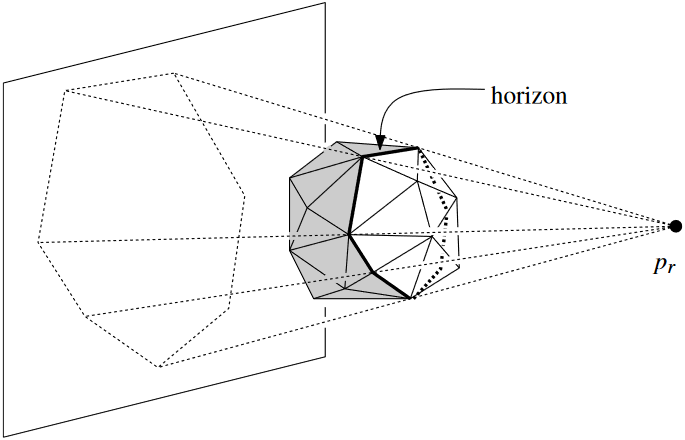
\includegraphics[width=0.45\textwidth]{higher_dim/threedim_visibility_horizon.png}
\caption{\label{fig:higher_dimensions_horizon} The dashed lines are the rays from the point $p_r$. The black edges are the horizon. The white faces are the faces visible from the point $p_r$ while the grey faces are on the other side of the horizon, so are not visible. This figure is from the book \cite{computgeombook}.}
\end{figure}

\newpage
\subsection{Conflict graph}
Given a set of points, the conflict graph allows to keep track of what faces are visible from a point that has not yet been processed. We have a vertex for each point and a vertex for every face of the convex hull. We have an edge between a point $p$ and a face $f$ if the face is visible from the point. The edges are called conflicts because if we want to add $p$ to the convex hull, we have to remove $f$ and all the faces that $p$ can see and we have to add the edges from $p$ to any point in $p$'s horizon.

\begin{figure}[h]
\centering
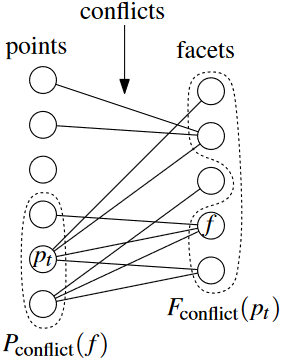
\includegraphics[width=0.25\textwidth]{higher_dim/conflict_graph.png}
\caption{\label{fig:conflict_graph} Graphical representation of a conflict graph: the points are the left nodes, the faces are the right nodes and the edges are the conflicts. Here the point $p_t$ can see the face $f$ and other 3 faces, while the face $f$ is visible from $p_t$ and other 2 points. Figure from the book \cite{computgeombook}.}
\end{figure}

Given a point $p_t$ and a face $f$, we can define two useful functions, $P_{conflict}(f)$ and $F_{conflict}(p_t)$. $F_{conflict}(p_t)$ is the set of faces that are visible from the point $p_t$. $P_{conflict}(f)$ is the set of points that can see the face $f$.

\subsection{Incremental algorithm}

The Incremental convex hull algorithm can be extended to compute the convex hull of a set of points in N-dimensions. It is slower than the others but it is preferred in practice. The algorithm starts with a minimal convex hull (for example in 3D is a tetrahedron), then iterates through all the points and adds that points that lie outside of the convex hull. To work in higher dimensions, the approach differs in some steps. First thing first, the algorithm doesn't initially sort the points because it selects the next point randomly. Then, for each point, it checks if the point is outside the convex hull by computing the visible faces from the point. 

\begin{figure}[h]
\centering
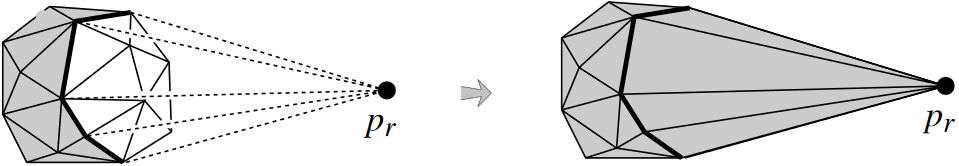
\includegraphics[width=0.7\textwidth]{higher_dim/incremental_3d_visual.png}
\caption{\label{fig:incremental_3d_visual}Example of one iteration of the incremental convex hull algorithm applied to a 3-dimensional set of points. The figure is inspired by the book \cite{computgeombook}.}
\end{figure}

If the point lies outside, then it is added to the convex hull, the edges connecting the point with the convex hull are also added to it and the faces that became inside the convex hull are removed. The algorithm stops until there are no remaining points. The key of the algorithm is how it computes the faces visible from a point and how it stores the points and the faces to efficiently compute the faces to be removed when a point is added to the hull.

\subsection{QuickHull}

N-dimensional Quickhull was invented in 1996 by C. Bradford Barber, David P. Dobkin, and Hannu Huhdanpaa \cite{quickhull3D}. It does not differ too much from the 2-dimensional case but it is an extension of it. As we know the algorithm begins by computing an initial hull. It does so in higher dimensions but, for example in 3D, it initially computes a triangle, like in the 2D version, and then it finds the furthest point from the triangle plane. This creates an initial hull which has the shape of a tetrahedron. 

Then the algorithm partitions the remaining points into the conflict lists of the faces of the initial hull. It iteratively adds new points to the hull by selecting the points with the largest distance from the conflicts. This involves the computation of the selected point's horizon. For each horizon edge, the algorithm creates a face and adds it to the hull. At this step some faces have been closed inside the convex hull, so the algorithm removes them. It continues selecting the points until there are no remaining points.

\subsection{Chan's algorithm}

Chan's paper about its algorithm for computing the convex hull also describes the approach for higher dimensions. As we know, Chan's algorithm uses Jarvis's march. In higher dimensions it uses higher-dimensional analogue of the gift wrapping algorithm. However, the algorithm in 2-dimensional space also uses Graham's scan, which cannot be extended to work in higher dimensions. It is replaced by the higher dimensions version of the Divide and Conquer algorithm by Preparata. The rest of the algorithm and the overall idea behind it remains unchanged.

\subsection{Divide and conquer}

The Divide and conquer algorithm by Preparata doesn't change too much when it is extended to compute the convex hull of a set of points in N-dimensions. As usual, the algorithm splits the point set into two sets, calls itself recursively in both sets and the merges the results. The following figure is a graphical representation of computing the convex hull in 3-dimensions.

\begin{figure}[h]
\centering
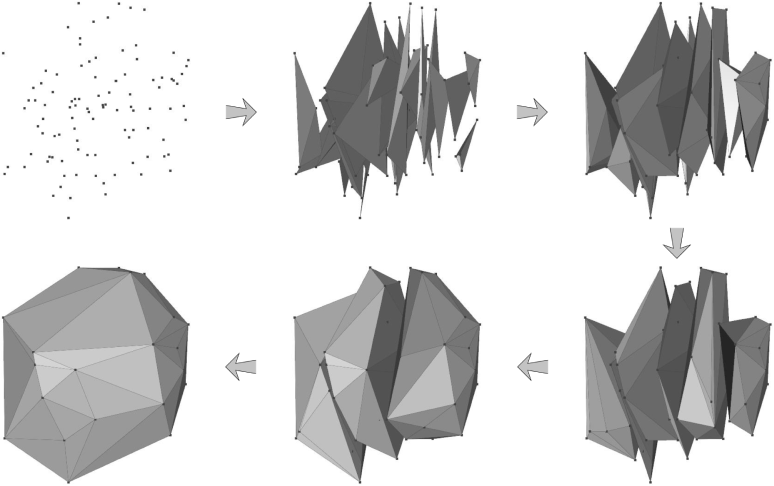
\includegraphics[width=0.5\textwidth]{higher_dim/divide_and_conquer_3d.png}
\caption{\label{fig:divide_and_conquer_3d}Example of Divide and conquer in 3-dimensions. Images from \cite{divideandconquer3d}}
\end{figure}

The key step of the algorithm is the merging phase. In higher dimensions it uses the gift wrapping approach as shown in the next figure. Initially it determines a supporting line of the convex hulls, by projecting the hulls in 2-dimensions and using the 2D algorithm. Then it uses the gift wrapping approach to create the additional faces to connect the subhulls. Finally, it removes the faces that became hidden.

\begin{figure}[h]
\centering
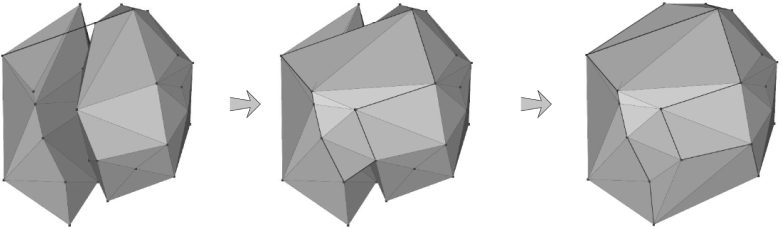
\includegraphics[width=0.5\textwidth]{higher_dim/divide_and_conquer_3d_merge.png}
\caption{\label{fig:divide_and_conquer_3d_merge} Merging phase of the divide and conquer algorithm in 3D. Images from \cite{divideandconquer3d}}
\end{figure}

\newpage
\section{Competitive programming problems}

\subsection{Wall (Easy)}
This is a simple competitive programming problem from the 2001-2002 ACM Northeastern European Regional Programming Contest and it available online on Timus Online Judge website \cite{wall_problem}.

\subsubsection*{Problem description}
A King ordered his chief Architect to build a wall around the King's castle. The King wants to build the wall around the whole castle using the least amount of stone and labor, but demanded that the wall should not come closer to the castle than a certain distance. The King demanded Architect to give the exact amount of resources that are needed to build the wall.
The task is to find the minimum possible length of the wall that the Architect could build around the castle to satisfy King's requirements.
The task is somewhat simplified by the fact, that the King's castle has a polygonal shape and is situated on a flat ground. The Architect has already established a Cartesian coordinate system and has precisely measured the coordinates of all castle's vertices in feet.

The input consists of $N$ pairs that represents the coordinates of the vertices in the King's castle and an integer which is the minimal number of feet that King allows for the wall to come close to the castle. All vertices are different and the sides of the castle do not intersect anywhere except for vertices.

\subsubsection*{Problem solution}
The castle is represented by a set of points, where each point is a vertex of the castle. In other words, this set of points is a polygon which can be convex or maybe not. It is easy to see that the optimal solution is the convex polygon that encloses the castle polygon. The reason is that the convex polygon in some way generalizes the shape of the castle with possibly less vertexes, walls, corners, etc. Computing it is, of course, computing the convex hull of the set of the castle's vertices and can be done with any algorithm.

Then, the remaining step is to "enlarge" the convex hull of the castle by the minimal amount desired by the King. Iterating through all the convex hull points and computing the sum of the distances between consecutive points is the optimal solution of the problem.

\subsection{Fence Orthogonality (Hard)}
This competitive programming problem is from the CTU Open 2013 contest and it is available online at open.kattis.com \cite{fence_orthogonality_problem}.

\subsubsection*{Problem description}
Evil bunnies are eating Freddy’s vegetables. In order to stop them, he decided to build a fence enclosing all vegetables in his garden. Freddy wants the fence to be as cheap (i.e., short) as possible, but for technical reasons, he can only build rectangular fences. For simplicity, we will assume the vegetables are negligibly small and can be represented by points in a two-dimensional plane.

The input consists of a first line with one integer N giving the number of vegetables in the garden. Each of the following N lines contains two integers, giving the coordinates of one vegetable to be protected. No two vegetables have the same coordinates. You may also assume the vegetables are not all on the same straight line.

\subsubsection*{Problem solution}

Given the vegetables in the garden as 2D points, the shortest fence enclosing all of them is of course their convex hull. But, if the fence must be a rectangle then it is the bounding box of the vegetables. A naïve approach is to simply take the smallest and largest x-coordinates e y-coordinates of the vegetables. This will certainly produce a rectangular bounding box. But, this approach computes a bounding box orthogonal to the axes and it is not always the minimum perimeter bounding box. By rotating the bounding box to any arbitrary angle, it is possible to find a rectangle that has the smaller perimeter.

It has been shown \cite{bb_collinear} that the minimum area bounding box of a set of points is collinear with one of the edges of the set's convex hull polygon.

\begin{figure}[h]
\centering
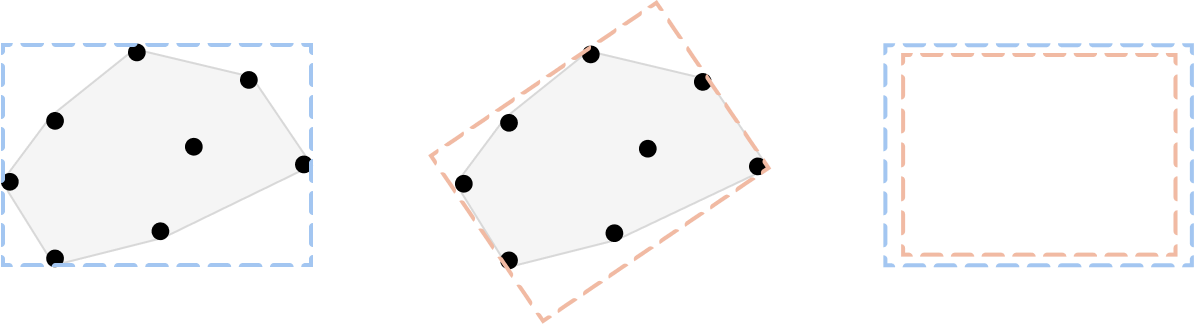
\includegraphics[width=0.7\textwidth]{competitiveprogramming/rotating_callipers.png}
\caption{\label{fig:rotating_callipers} Both rectangles are bounding boxes of the given points. The blue bounding box is orthogonal to the axes, but it has higher perimeter and area compared to the orange one. The minimum perimeter/area bounding box is also collinear with an edge of the convex hull.}
\end{figure}

The Rotating Calipers technique is a versatile method for solving a number of problems from the field of computational geometry and it can be used to solve this competitive programming problem. It is used to compute the diameter of convex polygons, minimum bounding box, minimum and maximum distance between two convex polygons, the intersection of convex polygons and many things more.

The first thing to do is to compute the convex hull of the vegetables and to find the bounding box orthogonal to the axes by computing the smallest and largest x-coordinates and y-coordinates. This also gives the initial minimum perimeter $P_{min}$. More formally, this bounding box is made by four supporting lines, each for each side. Then, rotate the supporting lines until one coincides with an edge of the convex hull, compute its perimeter and update the minimum perimeter $P_{min}$ and store the current rectangle if its perimeter is smaller than $P_{min}$. Repeat until any convex hull edge coincided at least one time with one of the supporting lines. 

The algorithm iterates through all the points and the computation for each iteration takes $O(1)$ time. Rotating can be done efficiently because at any step you know the next edge of the convex hull. Computing the perimeter is also trivial because at any step is known the base and height of the bounding box. So, the Rotating Calipers technique takes linear time to compute the minimal bounding box plus the time needed to compute the convex hull. 

\newpage
\section{Conclusion}

Not only in geometry and in competitive programming, but also in many other fields it is important to know about the convex hull and some of the strategies used by some algorithms can used to solve many other problems. The convex hull itself of a set of N-dimensional points gives a powerful tool to extrapolate many details about the set of points. Because of that, it has been studied for years by computer scientists and nowadays the convex hull is fundamental for many more computational geometry problems. The computation can be done with different approaches and there isn't one better than the others. For sure, it all depends of the intrinsic characteristics of the set of  points and their dimensionality.

The implementation of each algorithm is more or less trivial but it is important to efficiently store the convex hull and be as much smart as possible to lower the number of comparisons between points. Each algorithm has also its peculiarities and it is not possible to implement any of them by just looking to the pseudocode. The reason is that, because the problem is a geometric problem, it is needed a deep understanding of exactly what is happening and how during the iteration of each algorithm. Because of that, the pseudocode is a good starting point to understand how the algorithm compute the convex hull, but looking at an example visualization of each iteration of the algorithm is very important and it gives a deep and more clear understaing of how the algorithm works.

In the competitive programming world, a problem that just asks to compute the convex hull is not common because is a trivial problem: to solve it, it is just needed to know at least one algorithm for computing the convex hull. But, in competitive programming there are tons of problems that are geometric problems. To solve many of them it is required to compute the convex hull as the first or second step. This is why the convex hull problem is important for the competitive programming community.

Together with this report comes also a GitHub repository with all the source code of each algorithm, written in C++. It is available at \url{https://github.com/domferr/competitive-programming/tree/main/TheConvexHull}. Almost the entire source code can be read in this report, but the GitHub repository also contains a testsuite. Any algorithm has been unit tested with the testsuite by using the GoogleTest framework.

This report, its figures and the source code can also be a starting point for many other future projects. For example a web visualization of the computation of each algorithm, iteration after iteration. But also, extending the source code to compute the convex hull of 3-dimensional or N-dimensional set of points.

\newpage
\bibliographystyle{apalike}
\bibliography{bibliography}

\end{document}